% (The MIT License)
%
% Copyright (c) 2023-2024 Yegor Bugayenko
%
% Permission is hereby granted, free of charge, to any person obtaining a copy
% of this software and associated documentation files (the 'Software'), to deal
% in the Software without restriction, including without limitation the rights
% to use, copy, modify, merge, publish, distribute, sublicense, and/or sell
% copies of the Software, and to permit persons to whom the Software is
% furnished to do so, subject to the following conditions:
%
% The above copyright notice and this permission notice shall be included in all
% copies or substantial portions of the Software.
%
% THE SOFTWARE IS PROVIDED 'AS IS', WITHOUT WARRANTY OF ANY KIND, EXPRESS OR
% IMPLIED, INCLUDING BUT NOT LIMITED TO THE WARRANTIES OF MERCHANTABILITY,
% FITNESS FOR A PARTICULAR PURPOSE AND NONINFRINGEMENT. IN NO EVENT SHALL THE
% AUTHORS OR COPYRIGHT HOLDERS BE LIABLE FOR ANY CLAIM, DAMAGES OR OTHER
% LIABILITY, WHETHER IN AN ACTION OF CONTRACT, TORT OR OTHERWISE, ARISING FROM,
% OUT OF OR IN CONNECTION WITH THE SOFTWARE OR THE USE OR OTHER DEALINGS IN THE
% SOFTWARE.

\documentclass{article}
\usepackage{../sqm}
\newcommand*\thetitle{Code Coverage}
\begin{document}

\plush{\sqmTitlePage{15}{pJrXQ5rptig}}

\pptBanner{Example, Part I}
\begin{multicols}{2}
Live Code:\par
{\small\begin{ffcode}
(*@\textcolor{green}{int fibonacci(int n) \{} @*)
  (*@\textcolor{green}{if (n <= 0) \{} @*)
    return 0;
  (*@\textcolor{green}{\}} @*)
  (*@\textcolor{green}{if (n <= 2) \{} @*)
    (*@\textcolor{green}{return 1;} @*)
  (*@\textcolor{green}{\}} @*)
  return fibonacci(n-1)
    + fibonacci(n-2);
(*@\textcolor{green}{\}}@*)
\end{ffcode}
}
\par\columnbreak\par
Test Code:\par
{\small\begin{ffcode}
assert fibonacci(1) == 1;
assert fibonacci(2) == 1;
\end{ffcode}
}
\( C = 7/10 = 70\% \)
\end{multicols}
\plush{}

\pptBanner{Example, Part II}
\begin{multicols}{2}
Live Code:\par
{\small\begin{ffcode}
(*@\textcolor{green}{int fibonacci(int n) \{} @*)
  (*@\textcolor{green}{if (n <= 0) \{} @*)
    return 0;
  (*@\textcolor{green}{\}} @*)
  (*@\textcolor{green}{if (n <= 2) \{} @*)
    (*@\textcolor{green}{return 1;} @*)
  (*@\textcolor{green}{\}} @*)
  (*@\textcolor{green}{return fibonacci(n-1)}@*)
    (*@\textcolor{green}{+ fibonacci(n-2);}@*)
(*@\textcolor{green}{\}}@*)
\end{ffcode}
}
\par\columnbreak\par
Test Code:\par
{\small\begin{ffcode}
assert fibonacci(1) == 1;
assert fibonacci(2) == 1;

assert fibonacci(9) == 34;
assert fibonacci(10) == 55;
\end{ffcode}
}
\( C = 9/10 = 90\% \)
\end{multicols}
\plush{}

\pitch{\pptBanner{Some Kinds of Code Coverage}
\begin{itemize}\setlength\itemsep{0em}
\item Line Coverage
\item Statement Coverage
\item Branch Coverage
\item Condition Coverage
\item Function Coverage
\item Linear Code Sequence and Jump (LCSAJ) Coverage
\item Modified Condition / Decision Coverage (MC/DC)
\end{itemize}}

\pptBanner{Four Kinds of Coverage}
\begin{multicols}{2}
Live Code:\par
{\small\begin{ffcode}
int foo(int x) {
  if (x < 0) { return x; }
  if (x > 10 || x == 0) {
    return 42 / x;
  } else {
    return 1;
  }
}
\end{ffcode}
}
\par\columnbreak\par
Test Code:\par
{\small\begin{ffcode}
assert foo(1) == 1;
assert foo(50) == 42;
\end{ffcode}
}
\( C_{\texttt{line}} = 6/6 = 100\% \)\par
\( C_{\texttt{statement}} = 5/6 = 83\% \)\par
\( C_{\texttt{branch}} = 3/4 = 75\% \)\par
\( C_{\texttt{condition}} = 3/5 = 60\% \)\par
\end{multicols}
\plush{}

\qte
  [William Robert Elmendorf]
  {william-elmendorf}
  {A disciplined test control process is composed of five steps: 1) establish the intended extent of testing; 2) create a list of functional \ul{variations} eligible for testing; 3) rank and subset the \ul{eligible} variations so that test resources can be directed at those with the higher payoff; 4) calculate the \ul{test coverage} of the test case library; and 5) verify attainment of the \ul{planned} test coverage.}
  {elmendorf1969}

\qte
  [David Gelperin]
  {david-gelperin}
  {However, only half regularly document their test designs, only half regularly save their tests for reuse after software changes, and an extremely small five percent provide regular \ul{measurements} of code coverage.}
  {gelperin1988}

\plush{
\begin{multicols}{2}
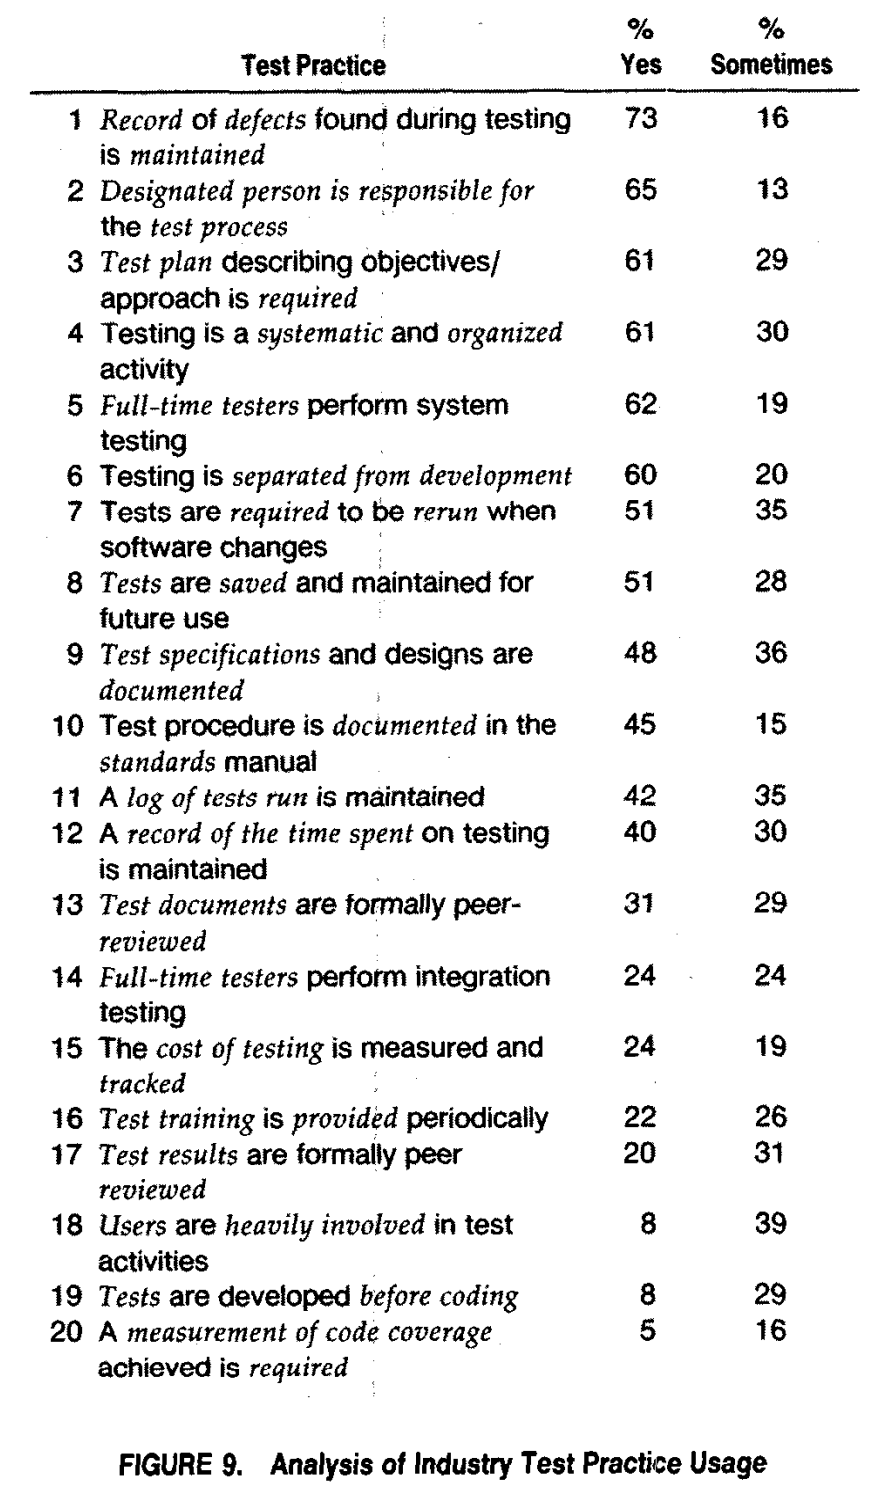
\includegraphics[width=.7\linewidth]{practices.png}
\par\columnbreak\par
``We note an \ul{inconsistency}. A high percentage of the respondents
felt that the testing in their organization was a systematic
and organized activity (91\% answered either ``yes''
or ``sometimes'' to this practice). However, [...]
an extremely small 5\% provide \ul{regular
measurements of code coverage}.''\par
{\scriptsize --- \textit{The Growth of Software Testing}, David Gelperin and Bill Hetzel, Communications of the ACM, 31(6), 1988\par}
\end{multicols}
}

\qte
  [Boris Beizer]
  {boris-beizer}
  {Junky software takes more tests to achieve coverage, but it breaks under any systematic test.}
  {beizer1995}

\qte
  [Brian Marick]
  {brian-marick}
  {Coverage numbers (like many numbers) are dangerous because they're \ul{objective} but \ul{incomplete}. They too often distort sensible action. Using them in isolation is as foolish as hiring based only on GPA.}
  {marick1997}

\qte
  [Martin Fowler]
  {martin-fowler}
  {I would be suspicious of anything like 100\% --- it would smell of someone writing tests to make the coverage \ul{numbers happy}, but not thinking about what they are doing.}
  {fowler1997}

\qte
  [Cem Kaner]
  {cem-kaner}
  {As you get near 100 percent line coverage, that doesn't tell you the product is near release. It just tells you that the product is no longer \ul{obviously far} from release according to \ul{this measure}.}
  {kaner2002}

\qte
  [Pavneet Singh Kochhar, David Lo, Julia Lawall, Nachiappan Nagappan]
  {pavneet-singh-kochhar}
  {Our results show that coverage has an \ul{insignificant correlation} with the number of bugs that are found after the release of the software at the project level, and \ul{no such correlation} at the file level.}
  {kochhar2017}

\qte
  [Goran Petrovi{\'c}]
  {goran-petrovic}
  {Google \ul{does not enforce} any code coverage thresholds across the entire codebase. Projects (or groups of projects) are free to define their own thresholds and goals. Many projects opt-into a centralized voluntary alerting system that defines \ul{five levels} of code coverage thresholds.}
  {ivankovi2019}


\pitch{\pptBanner{Code Coverage Threshold Levels in Google}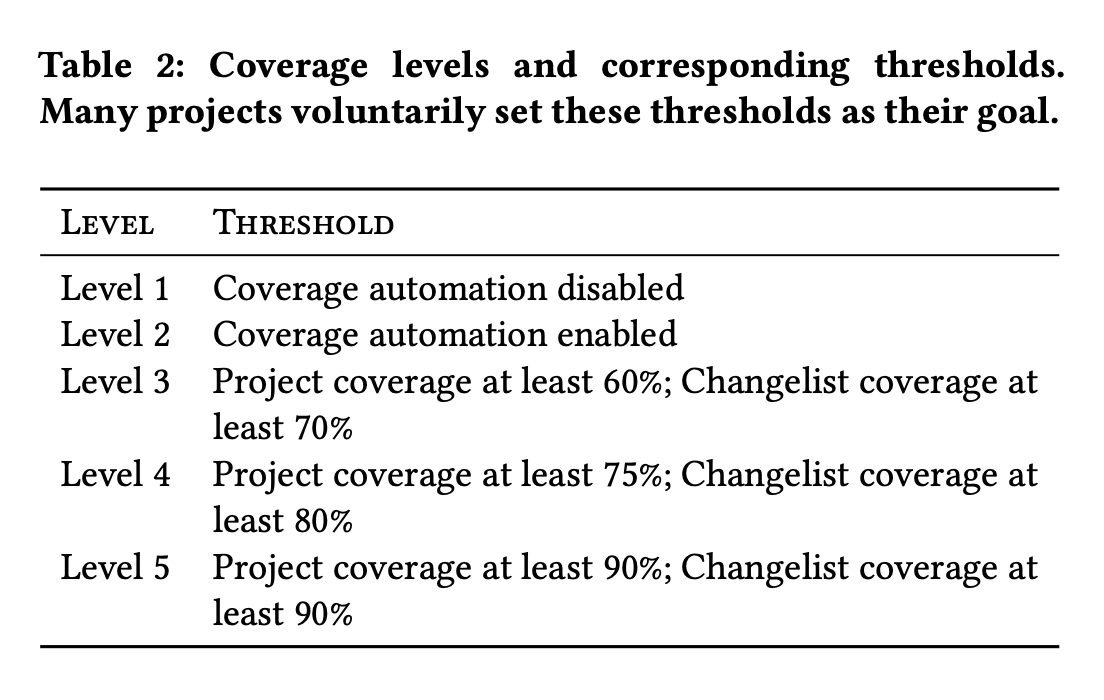
\includegraphics[width=.7\textwidth]{levels.png}}

\qte
  [Adam Bender]
  {adam-bender}
  {Code coverage \ul{does not guarantee} that the covered lines or branches have been tested correctly, it just guarantees that they have been executed by a test. But a low code coverage number \ul{does guarantee} that large areas of the product are going completely untested by automation on every single deployment.}
  {arguelles2020}

\qte
  {../15-code-coverage/survey}
  {Many \ul{contracts} are specifying that a certain \ul{percentage} of the statements or instructions must be successfully executed before the acceptance of the software by the customer.}
  {bowen1979survey}

\pitch{\pptBanner{Industry Standards that Require Code Coverage}
\begin{itemize}
\item ISO-26262: ``Road Vehicles'' functional safety (Switzerland)
\item IEC 61508: ``Functional Safety of Electrical/Electronic/Programmable Electronic Safety-related Systems'' (UK)
\item DO-178C: ``Software Considerations in Airborne Systems and Equipment Certification'' (USA)
\item IEC 62304: ``Medical Device Software'' (UK)
\end{itemize}}

\pitch{
\begin{pptWide}{2}
ISO-26262:\\
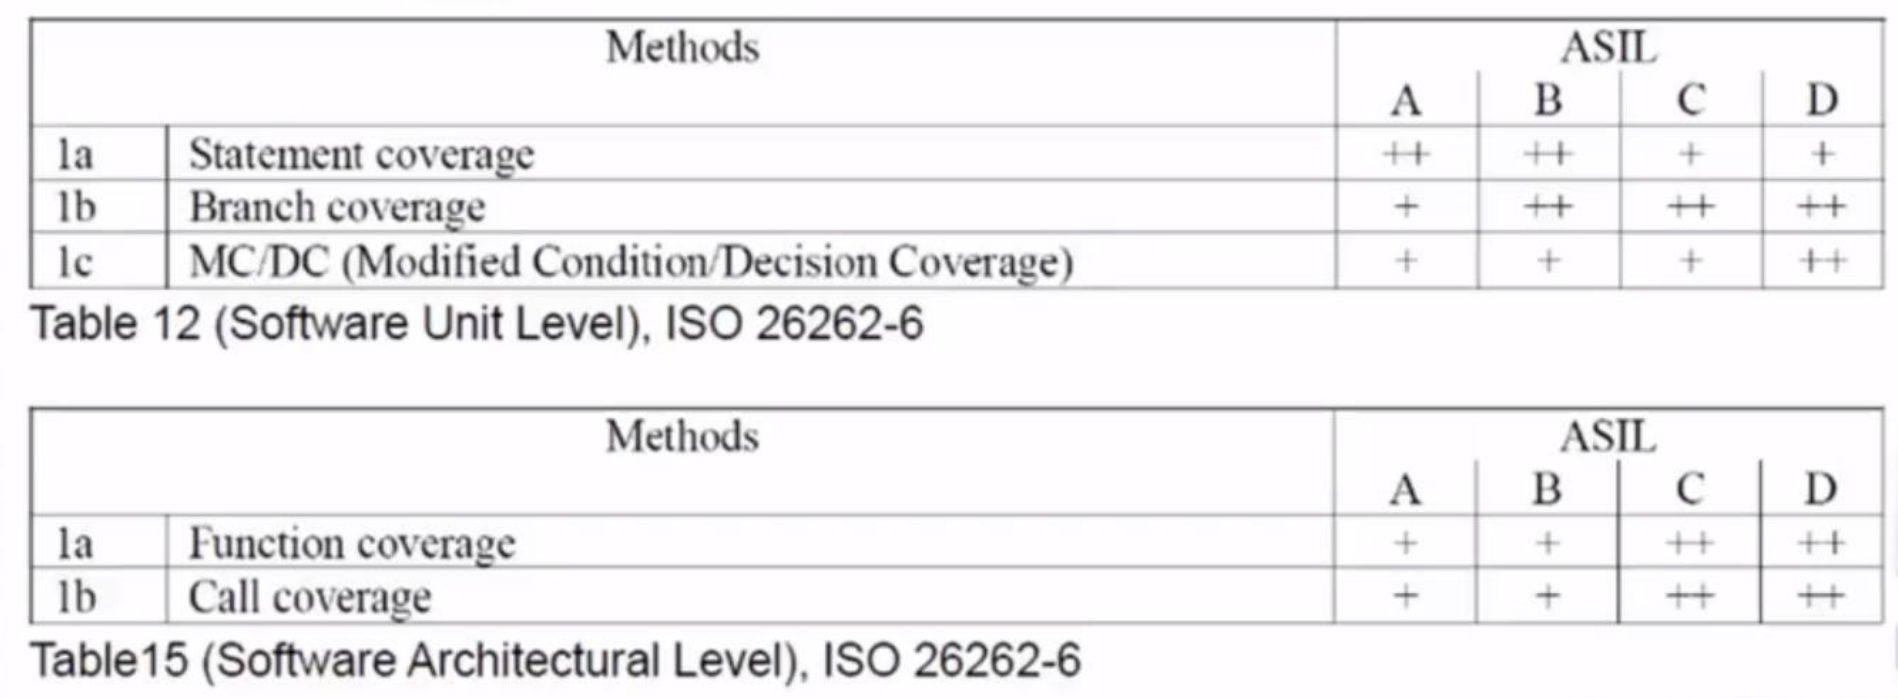
\includegraphics[width=.9\linewidth]{iso-26262.png}\par
IEC 61508:\\
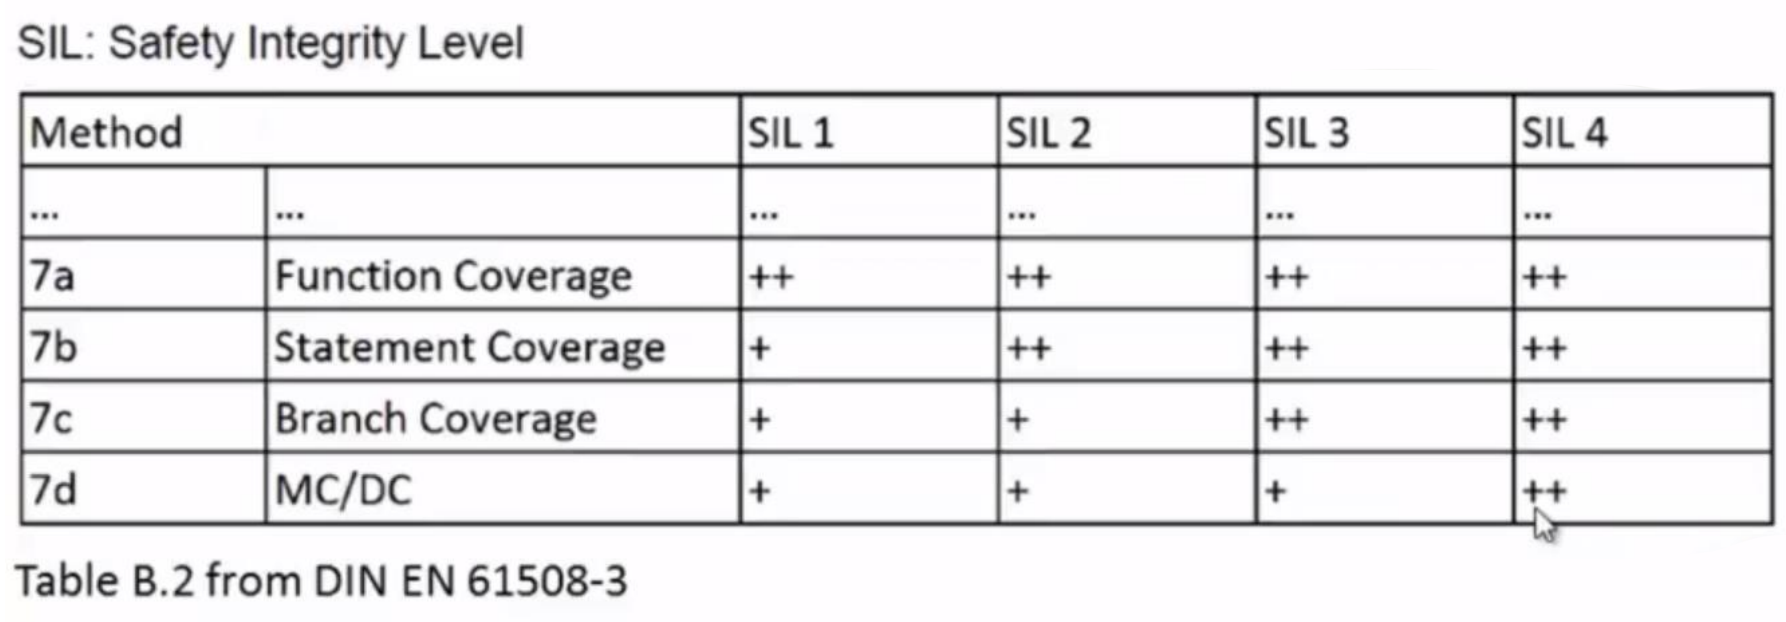
\includegraphics[width=.9\linewidth]{iec-61508.png}\par
\par\columnbreak\par
DO-178C:\\
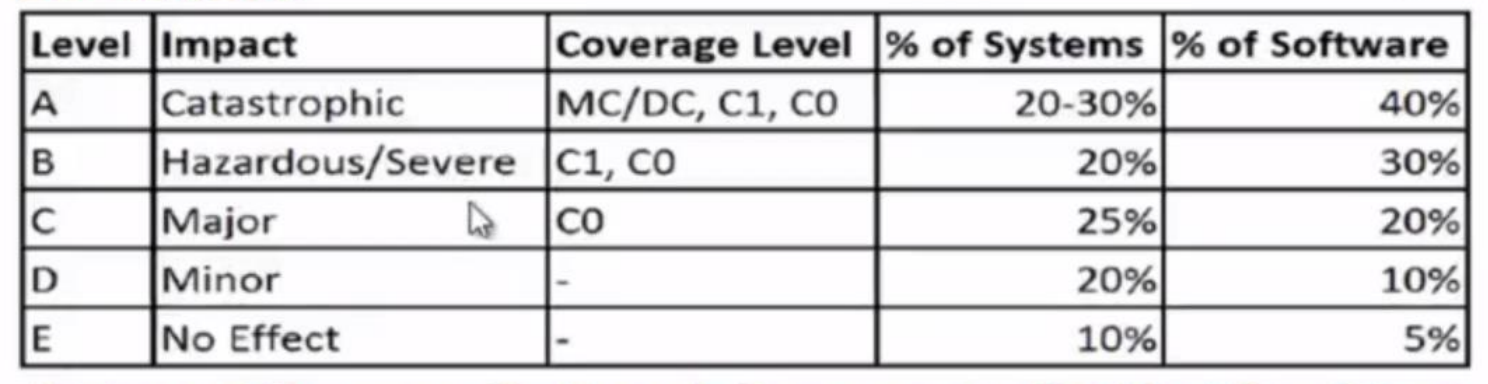
\includegraphics[width=.9\linewidth]{do-178c.png}\par
IEC 62304:\\
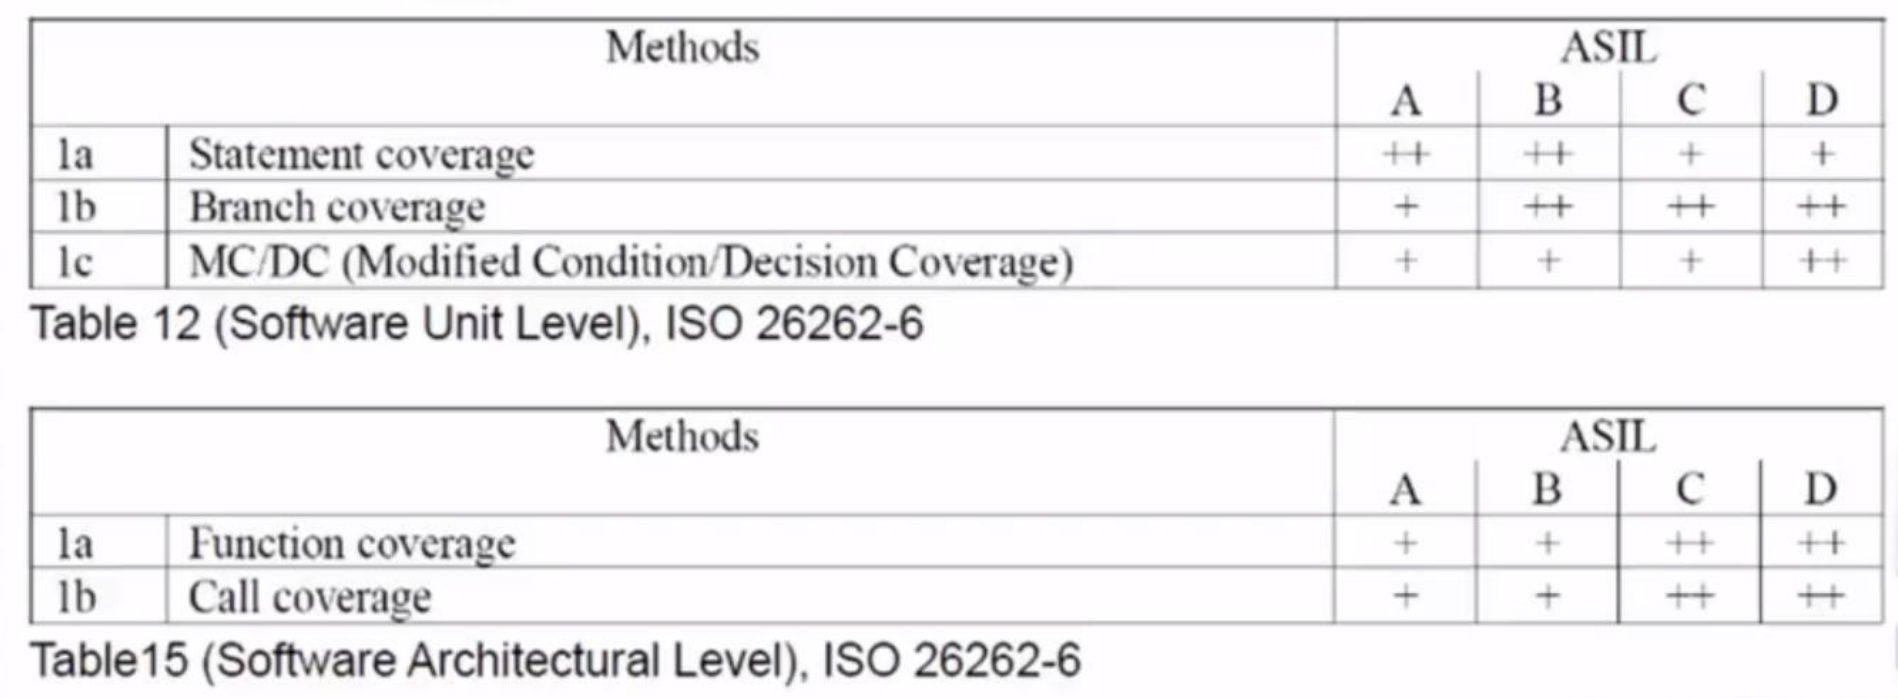
\includegraphics[width=.9\linewidth]{iso-26262.png}\par
\end{pptWide}
}

\pitch{\pptBanner{Codecov.io}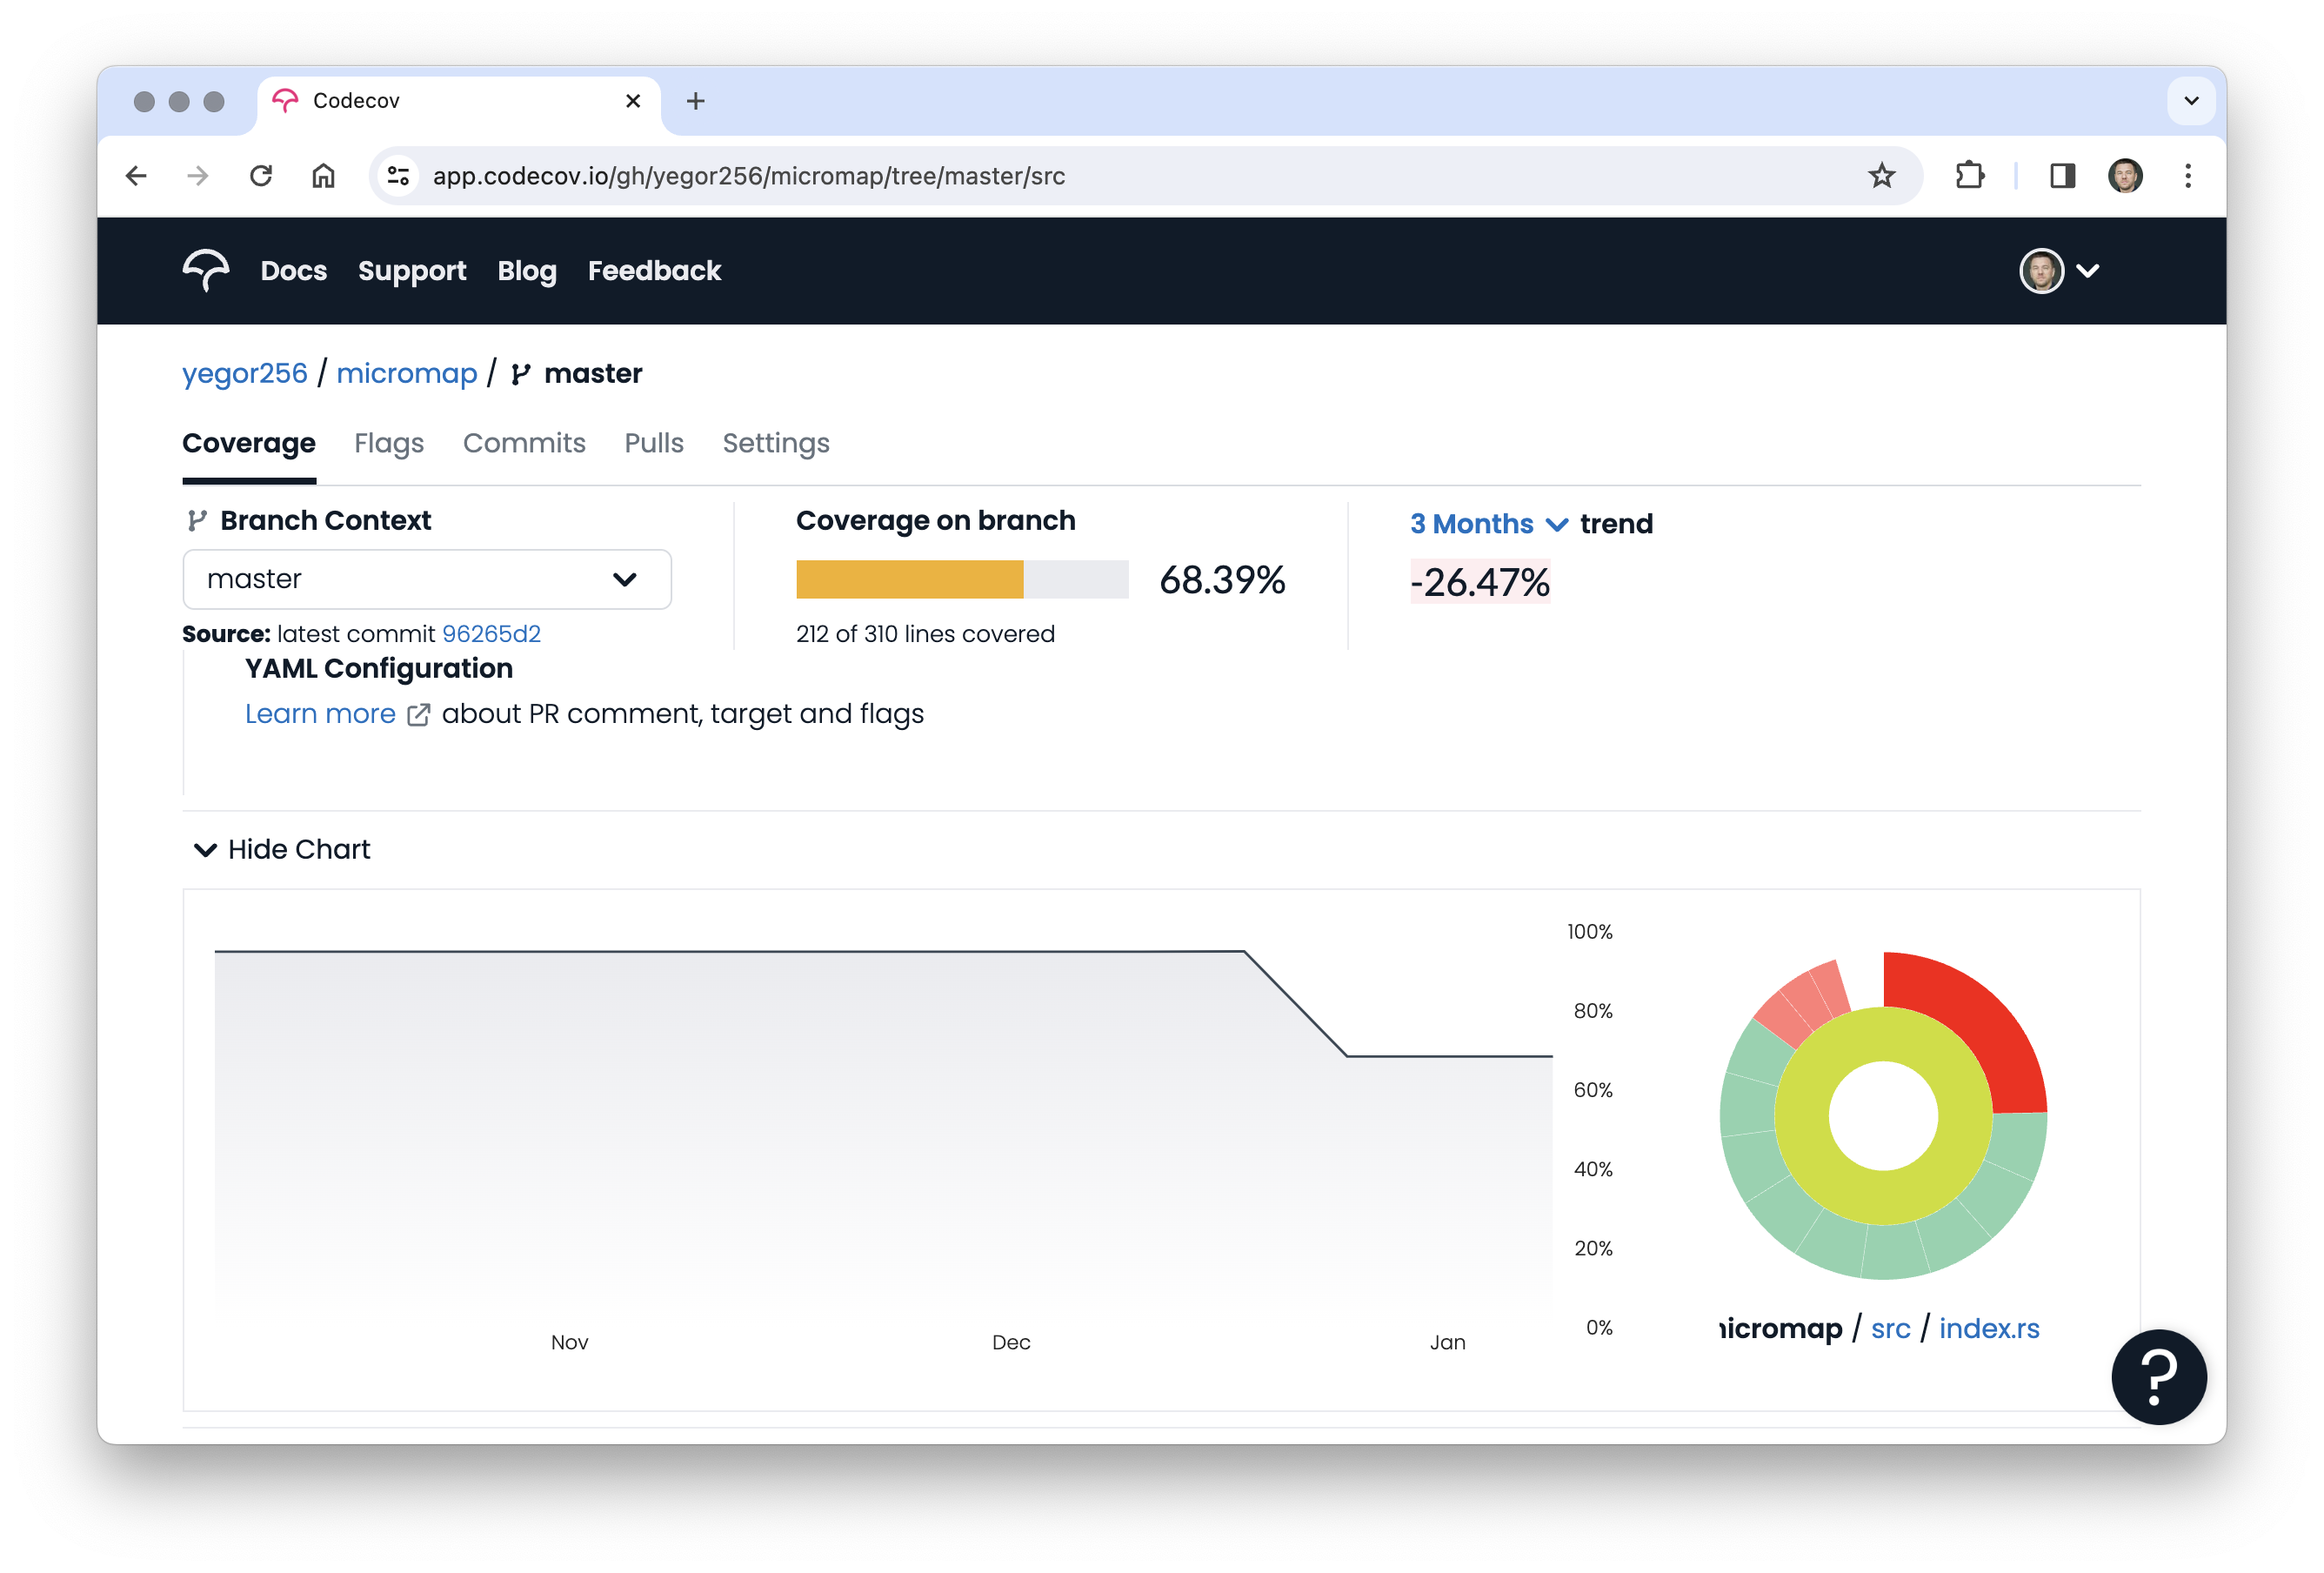
\includegraphics[width=.7\textwidth]{codecov.png}}

\pitch{\pptBanner{Line Coverage}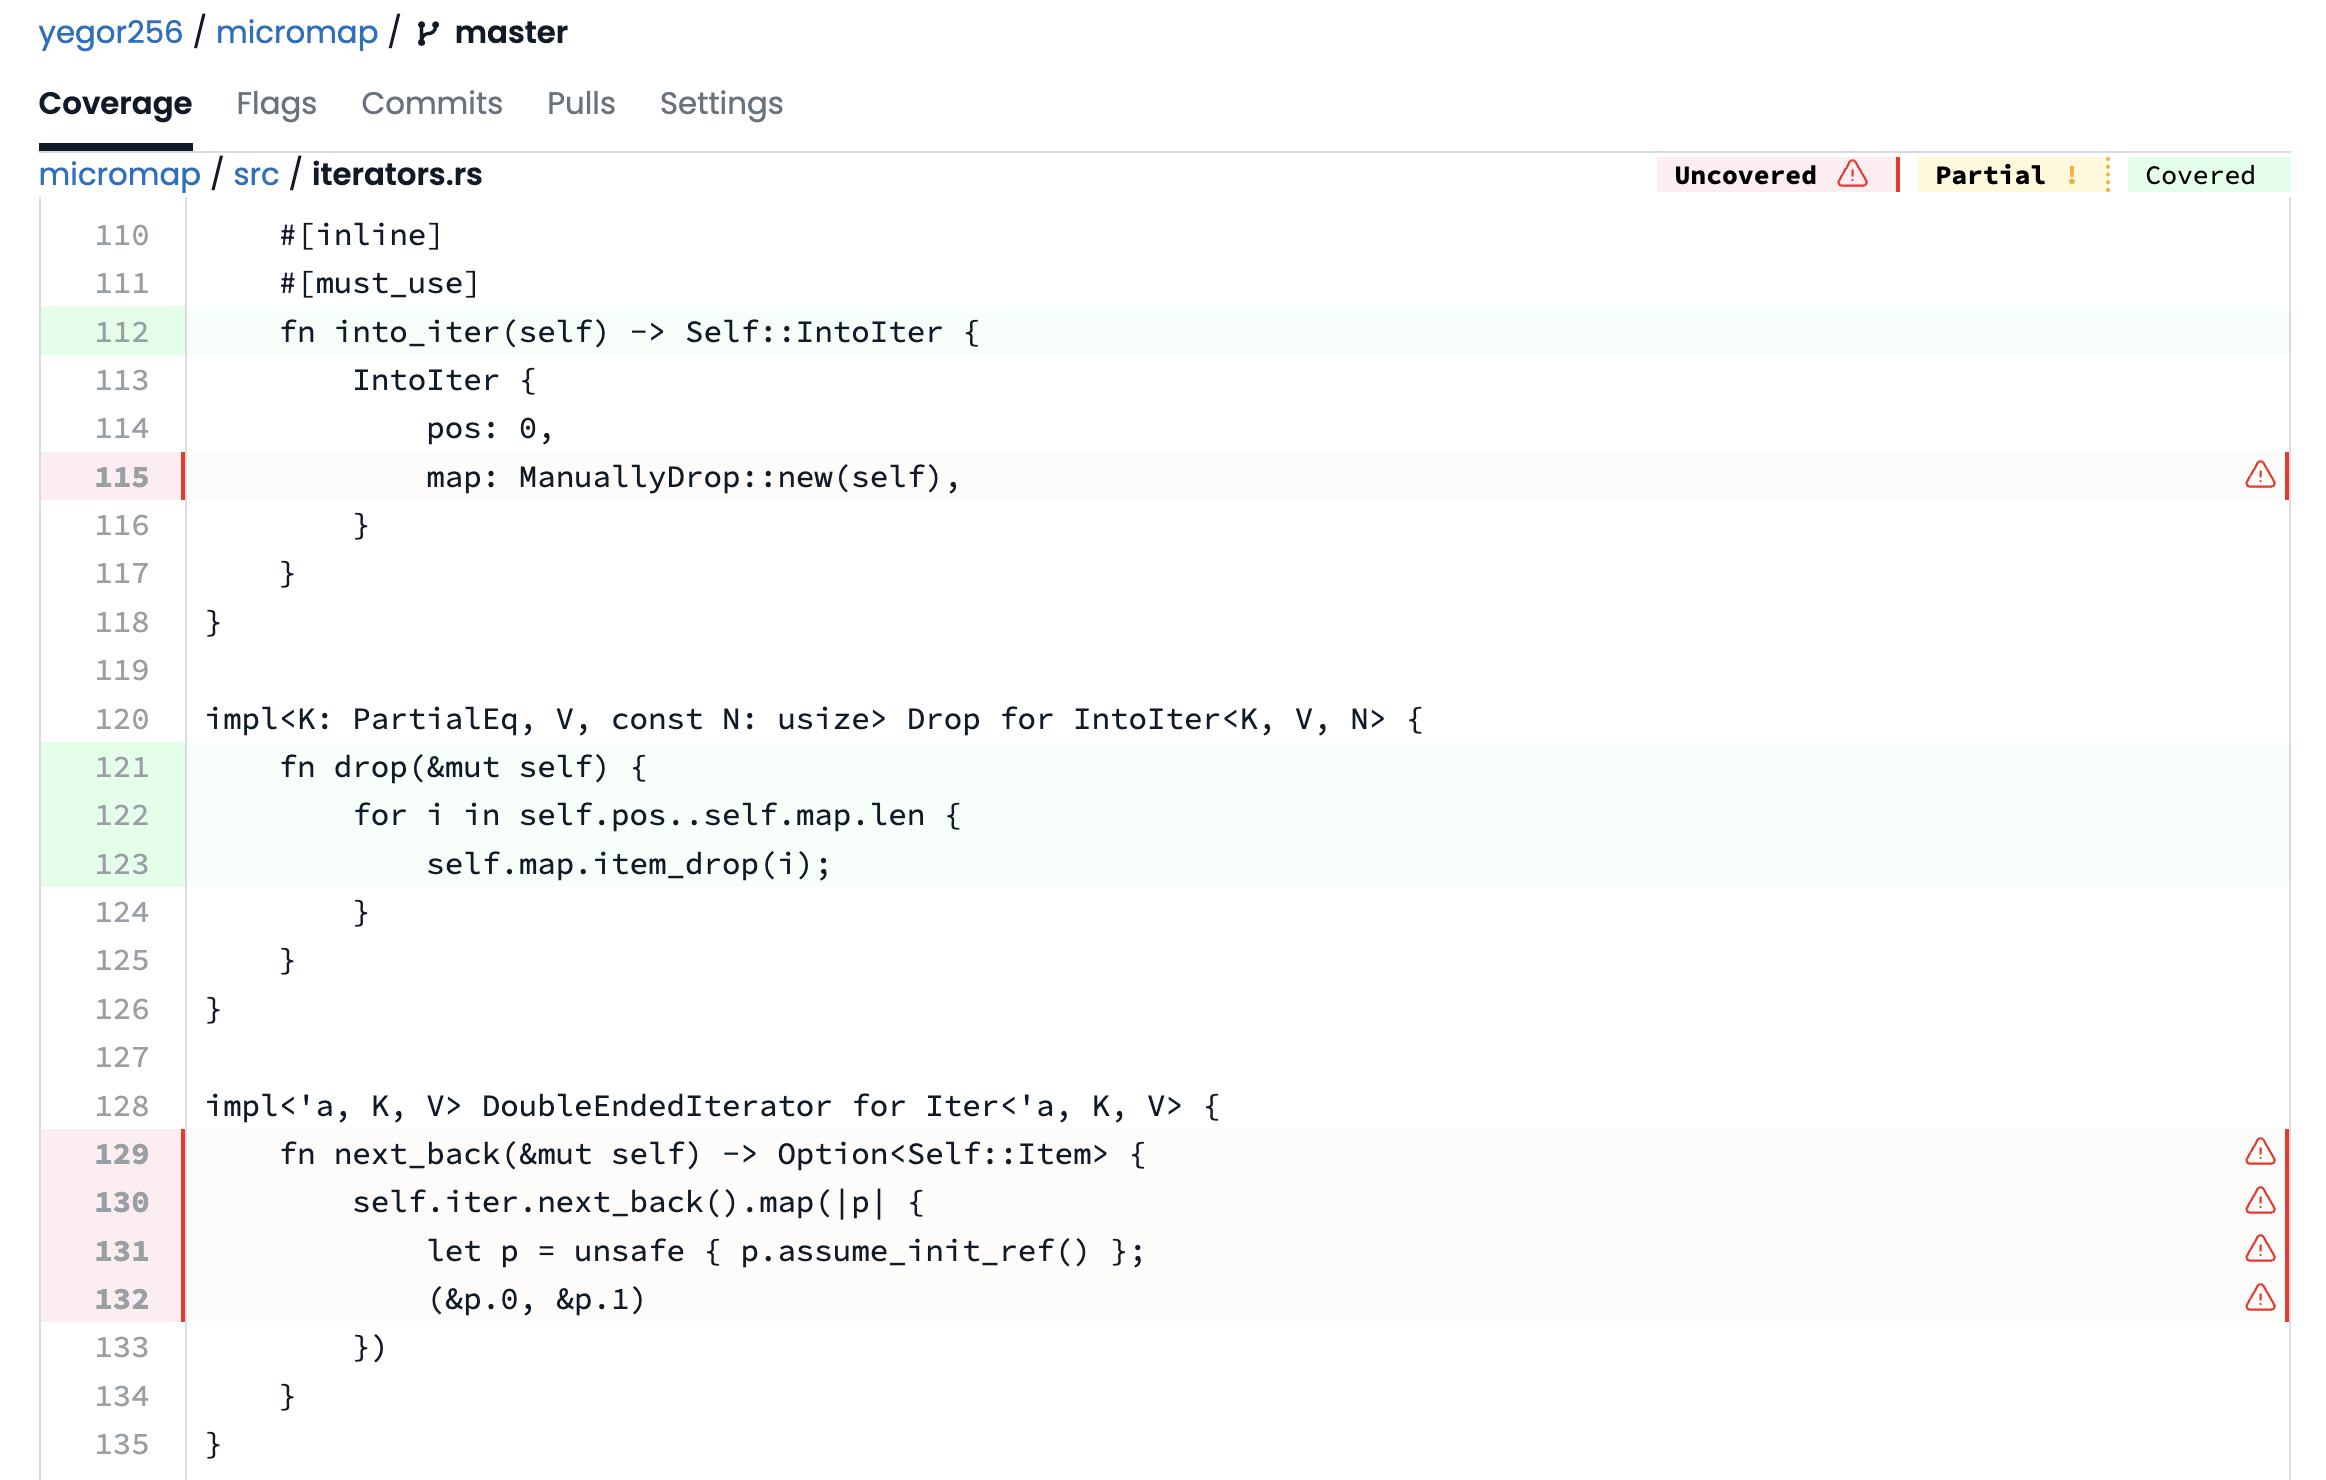
\includegraphics[width=.7\textwidth]{lines.png}}

\pitch{\pptBanner{Tarpaulin for Rust}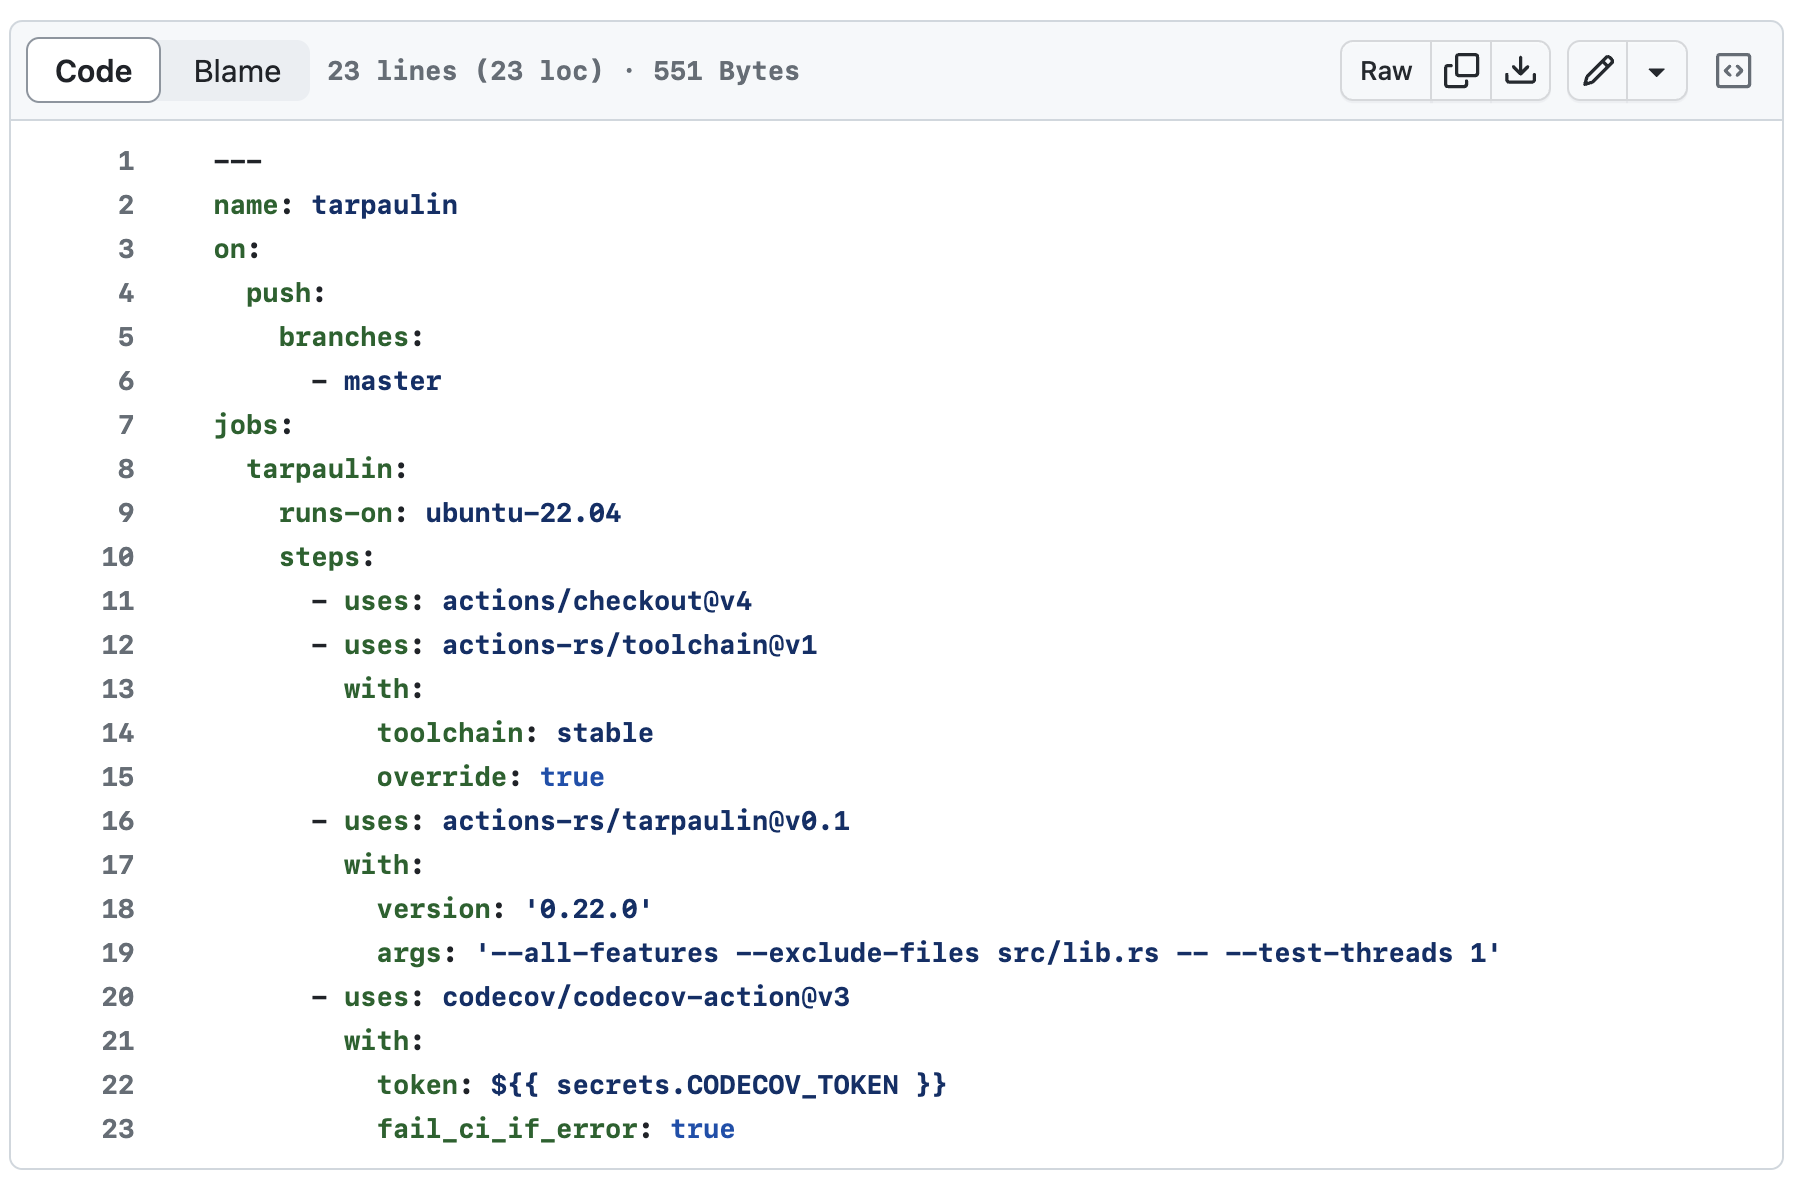
\includegraphics[width=.7\textwidth]{tarpaulin.png}}

\pptBanner{Code Coverage Threshold, JaCoCo Example}
\begin{multicols}{2}
{\tiny\begin{ffcode}
<project>
  [...]
  <build>
    <plugins>
      <plugin>
        <groupId>org.jacoco</groupId>
        <artifactId>jacoco-maven-plugin</artifactId>
        <version>0.8.11</version>
        <executions>
          <execution>
            <id>jacoco-initialize</id>
            <goals>
              <goal>prepare-agent</goal>
            </goals>
          </execution>
          <execution>
            <id>jacoco-check</id>
            <goals>
              <goal>check</goal>
            </goals>
            <configuration>
              <rules>
                (*@\textcolor{orange}{[...] \(\leftarrow\) Next slide}@*)
              </rules>
            </configuration>
          </execution>
          <execution>
            <id>report</id>
            <goals>
              <goal>report</goal>
            </goals>
          </execution>
        </executions>
      </plugin>
    </plugins>
  </build>
</project>
\end{ffcode}
}
\end{multicols}
\plush{}

\pptBanner{Code Coverage Threshold, JaCoCo Rules}
\begin{multicols}{2}
{\tiny\begin{ffcode}
<rules>
  <rule>
    <element>BUNDLE</element>
    <limits>
      <limit>
        <counter>(*@\textcolor{orange}{INSTRUCTION}@*)</counter>
        <value>COVEREDRATIO</value>
        <minimum>0.67</minimum>
      </limit>
      <limit>
        <counter>(*@\textcolor{orange}{LINE}@*)</counter>
        <value>COVEREDRATIO</value>
        <minimum>0.84</minimum>
      </limit>
      <limit>
        <counter>(*@\textcolor{orange}{BRANCH}@*)</counter>
        <value>COVEREDRATIO</value>
        <minimum>0.47</minimum>
      </limit>
      <limit>
        <counter>(*@\textcolor{orange}{COMPLEXITY}@*)</counter>
        <value>COVEREDRATIO</value>
        <minimum>0.57</minimum>
      </limit>
      <limit>
        <counter>(*@\textcolor{orange}{METHOD}@*)</counter>
        <value>COVEREDRATIO</value>
        <minimum>0.76</minimum>
      </limit>
      <limit>
        <counter>(*@\textcolor{orange}{CLASS}@*)</counter>
        <value>MISSEDCOUNT</value>
        <maximum>2</maximum>
      </limit>
    </limits>
  </rule>
</rules>
\end{ffcode}
}
\end{multicols}
{\scriptsize Source: \url{https://github.com/volodya-lombrozo/jtcop}\par}
\plush{}

\pitch{Code Coverage can be calculated by a few tools:
\begin{itemize}
\item \href{https://www.jacoco.org}{JaCoCo} for Java
\item \href{https://istanbul.js.org/}{Istanbul} for Javascript
\item \href{https://gcc.gnu.org/onlinedocs/gcc/Gcov.html}{Gcov} for C/C++
\item \href{https://pypi.org/project/coverage/}{Coverage.py} for Python
\item \href{https://github.com/simplecov-ruby/simplecov}{Simplecov} for Ruby
\item \href{https://github.com/xd009642/tarpaulin}{Tarpaulin} for Rust
\end{itemize}}

\end{document}
